\section{Variantenstudie der Lösungsansätze}\label{resultate}
In diesem Abschnitt werden die Ergebnisse der Variantenstudie zu den Lösungsansätzen vorgestellt. Für die Lösungsansätze wurden unterschiedliche Transformationen und Quantisierungen getestet, welche die Kompressionsrate erhöhen. Im ersten Abschnitt \ref{resultate:loesung0} wird der Lösungsansatz des Adaptiven Subsamplings besprochen. In den folgenden Abschnitten \ref{resultate:loesung1} und \ref{resultate:loesung2} folgen die Resultate der Ansätze DCT und Prädiktive Kodierung.

\subsection{Lösungsansatz: Adaptives Subsampling} \label{resultate:loesung0}
Im Ist-Zustand führt der JHelioviewer nach der Dekompression ein adaptives Subsampling durch. Dieser Lösungsansatz führt das adaptive Subsampling vor der Datenübertragung durch und Kodiert die Daten mit Rar anstatt mit Gzip. Eine genauere Beschreibung des Ansatzes ist im Abschnitt \ref{konzept:loesung0} zu finden.

\begin{figure}[!htbp]
	\center
	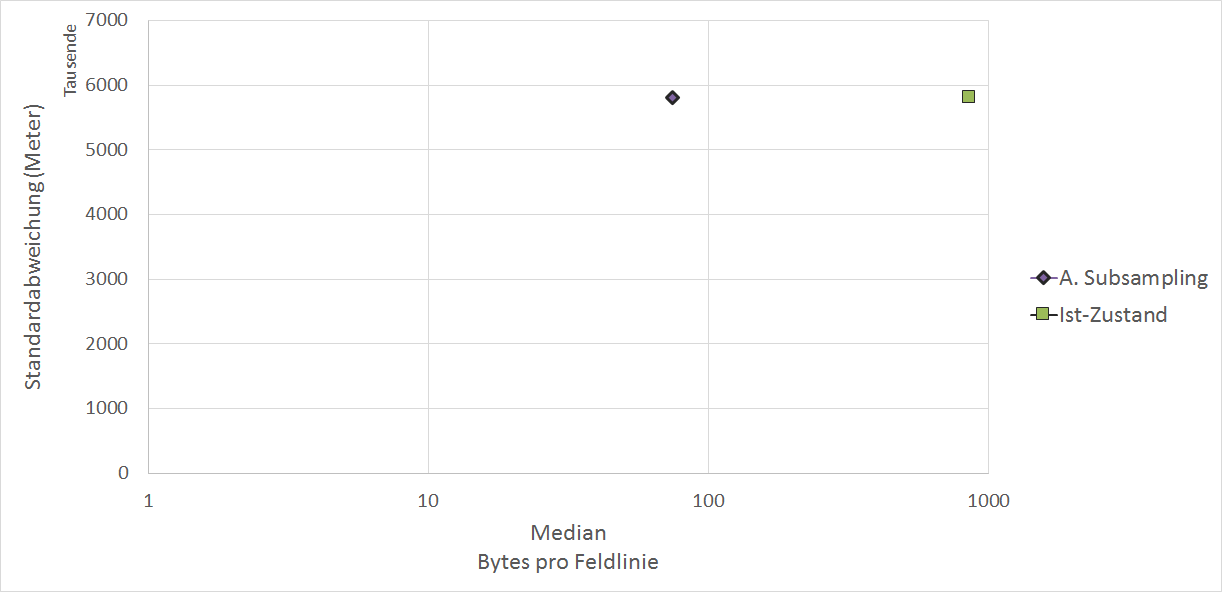
\includegraphics[width=1\textwidth,keepaspectratio]{./pictures/resultate/loesung0/loesung0_0.png}
	\caption{Vergleich des Lösungsansatzes: Adaptives Subsampling zur Ist-Kompression.}
	\label{resultate:loesung0:loesung0_0}
\end{figure}
Wie im Diagramm der Abbildung \ref{resultate:loesung0:loesung0_0} erkennbar ist, braucht dieser Lösungsansatz deutlich weniger Speicher als die Ist-Kompression zur selben Genauigkeit. Der Lösungsansatz des Adaptiven Subsamplings erreicht eine Kompressionsrate von $11.6$ gegenüber dem Ist-Zustand, indem es nur die Punkte überträgt, welche der JHelioviewers darstellt.

\begin{figure}[!htbp]
	\center
	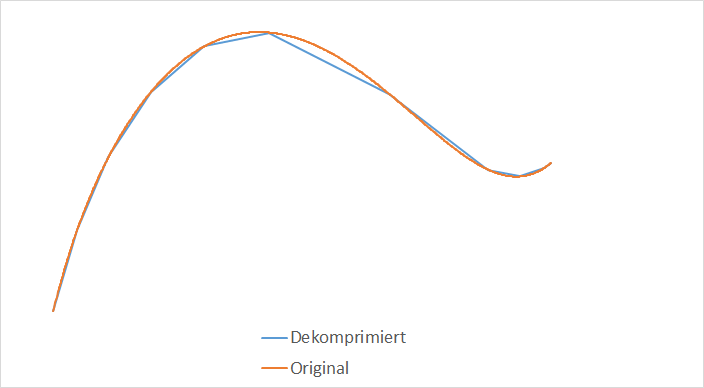
\includegraphics[width=1\textwidth,height=8cm,keepaspectratio]{./pictures/resultate/loesung0/loesung0_artefakte.png}
	\caption{Artefakte des Lösungsansatzes Adaptives Subsampling.}
	\label{resultate:loesung0:artefakte}
\end{figure}
Das Diagramm Abbildung \ref{resultate:loesung0:artefakte} zeigt die Artefakte der Kompression. Sie sind identisch mit den Artefakten der Visualisierung im Ist-Zustand. Die Artefakte sind in der JHelioviewer Visualisierung erst bei höheren Zoom-Stufen erkennbar.

Der JHelioviewer muss in der Lage sein $1000$ komprimierte Simulationen im Arbeitsspeicher abzulegen. Mit dieser Kompression werden durchschnittlich $85$ Megabyte an Arbeitsspeicher benötigt. Wenn von einer $10$ Megabit Internetverbindung ausgegangen wird, werden für das Herunterladen von $1000$ Simulationen $70$ Sekunden benötigt. Der Ist Zustand benötigt bei denselben Bedingungen $790$ Sekunden ($13$ Minuten) für die Übertragung. Mit dieser Kompression können etwa $14$ komprimierte Simulationen pro Sekunde übertragen werden. 

Ein Vorteil dieses Lösungsansatzes ist die Laufzeit Dekompression: Da keine rechenaufwändige Transformationen verwendet werden braucht dieser Lösungsansatz $19$ Millisekunden für eine Dekompression (Siehe Abschnitt \ref{anhang:performance}). Mit einem Thread ist die Testmaschine in der Lage $50$ Simulationen pro Sekunde zu dekomprimieren.

In Zukunft ist es möglich, dass im JHelioviewer deutlich mehr Punkte dargestellt werden sollen. In diesem Fall müssen entweder mehr Daten übertragen werden oder der JHelioviewer mit einer Interpolation erweitert werden.
\pagebreak
\subsection{Kompressionsverfahren: Diskrete Kosinus Transformation} \label{resultate:loesung1}
In diesem Abschnitt wird die Kompression mittels Diskreter Kosinus Transformation behandelt. Es wurden verschiedene Transformationen getestet, welche die Approximation mittels Kosinus Funktionen verbessern. Die Ableitung der Feldlinien dämpft die Kompressionsartefakte und ist massgebend für die Kompressionsrate verantwortlich.\\
Um die Feldlinien optimal mit der DCT zu approximieren, müssen Ringing-Artefakte, behandelt werden. Das Auftreten der Artefakte wird im Abschnitt \ref{resultate:loesung1:ringing} und die Behandlung im Abschnitt \ref{resultate:loesung1:behandlung_ringing} besprochen.

\subsubsection{Variante: DCT}\label{resultate:dct}

\begin{figure}[!htbp]
	\center
	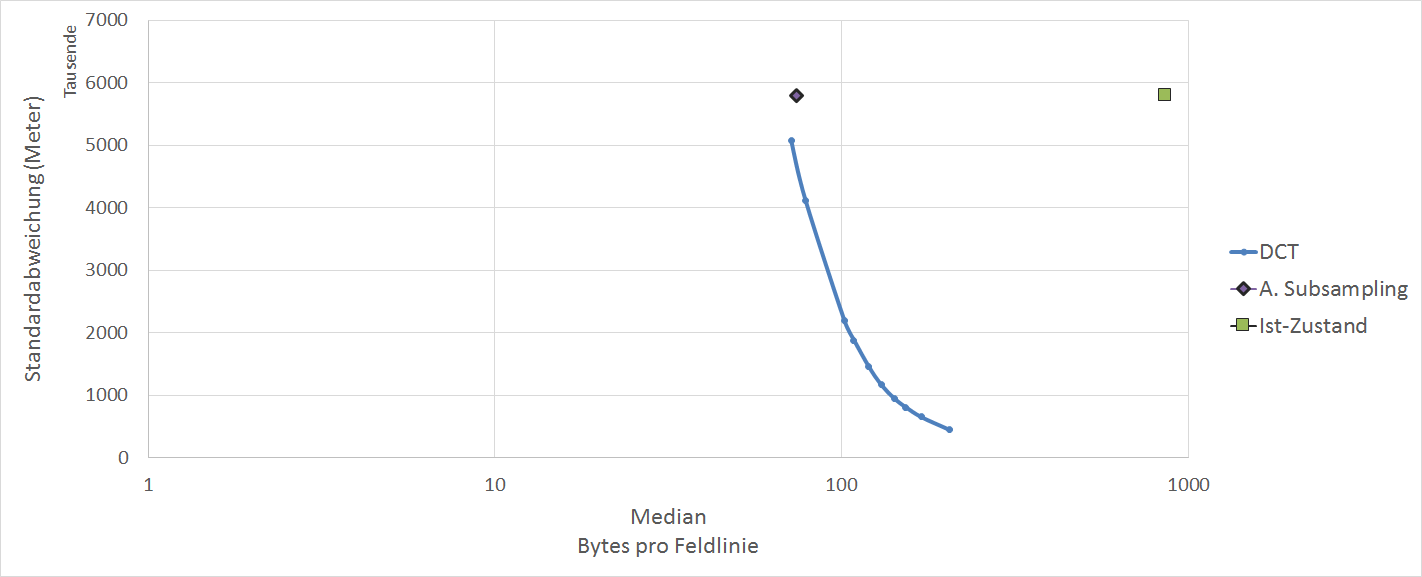
\includegraphics[width=1\textwidth,keepaspectratio]{./pictures/resultate/loesung1/loesung1-0/loesung1_0.png}
	\caption{Vergleich der DCT Kompression mit dem Verfahren des Adaptiven Subsamplings}
	\label{resultate:loesung1:dct:resultate}
\end{figure}
Die Abbildung \ref{resultate:loesung1:dct:resultate} zeigt den Vergleich der DCT Kompression mit dem Verfahren des Adaptiven Subsamplings (siehe \ref{resultate:loesung0}). Die Standardabweichung steigt mit stärkerer Quantisierung unerwartet schnell an. Der Grund dafür kann im Diagramm der Abbildung \ref{resultate:loesung1:dct:artefakte} entnommen werden:

\begin{figure}[!htbp]
	\center
	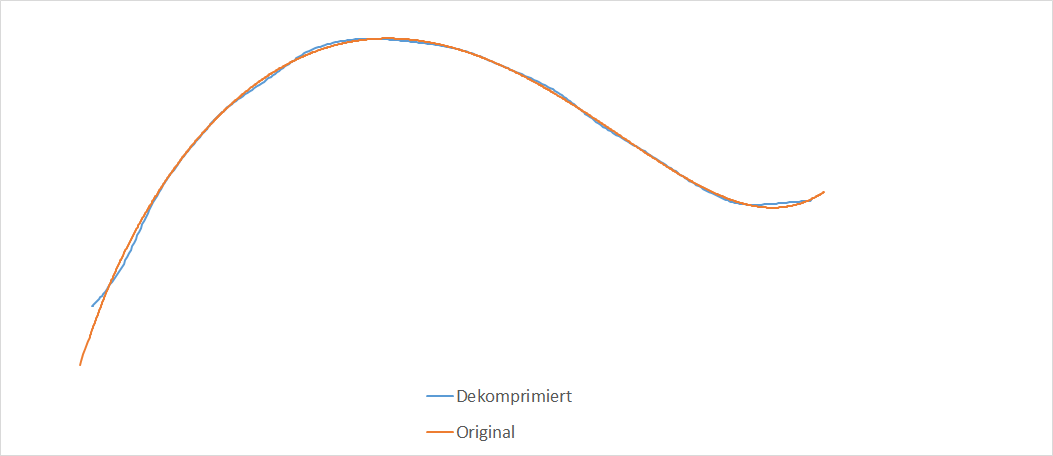
\includegraphics[width=0.8\textwidth,height=8cm,keepaspectratio]{./pictures/resultate/loesung1/loesung1-0/loesung1_0_artefakte.png}
	\caption{Artefakte der DCT Dekompression anhand Beispieldaten}
	\label{resultate:loesung1:dct:artefakte}
\end{figure}
Der Anfang und das Ende der Feldlinie können nicht gut approximiert werden. Dies ist ein typisches Problem der DCT: Ein Inputsignal wird in der DCT konzeptionell repetiert, da die DCT nur ein periodisches Signal transformieren kann. Dazu wird konzeptionell das Signal gespiegelt. Das Diagramm der Abbildung \ref{resultate:loesung1:dct:spiegelung} illustriert das Problem. Bei der Beispielfeldlinie aus Abbildung \ref{resultate:loesung1:dct:artefakte} führt die Wiederholung zu einer Spitze im Signal. Die Spitze wird in der DCT mit hochfrequenten Anteilen abgebildet, welche von der Quantisierung gelöscht werden. Das Ergebnis ist eine Verschiebung an den Stellen, wo die Spitze auftritt. In diesem Fall ist es jeweils am Anfang und am Ende der Feldlinie.

\begin{figure}[!htbp]
	\center
	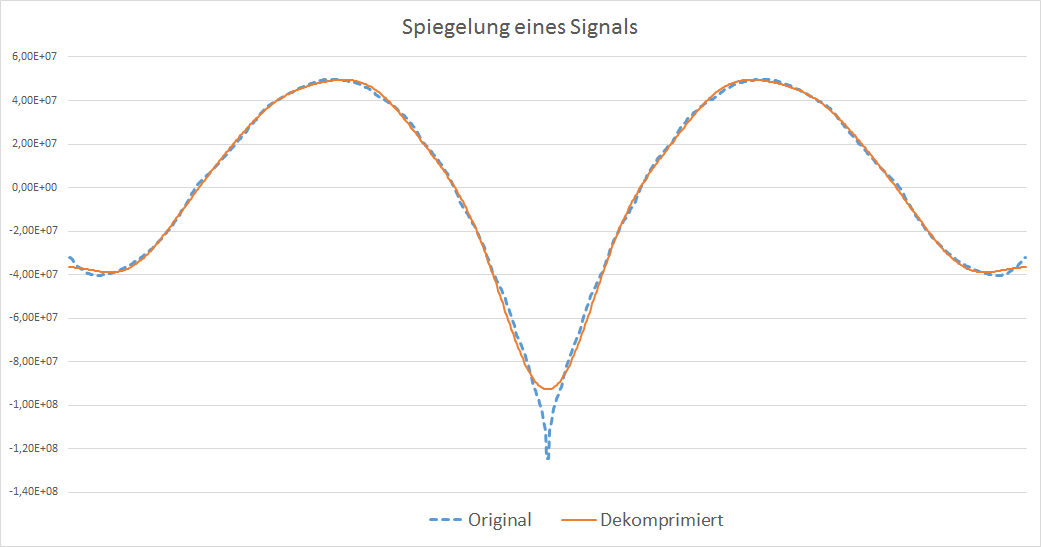
\includegraphics[width=0.8\textwidth,height=8cm,keepaspectratio]{./pictures/resultate/loesung1/loesung1-0/spiegelung.png}
	\caption{Konzeptionelle Spiegelung an den Rändern des Signals.}
	\label{resultate:loesung1:dct:spiegelung}
\end{figure}
Das Problem kann entweder durch eine vorhergehende Transformation der Feldlinie oder durch zusätzliche Daten am Anfang und am Ende der Linie gelöst werden. Die Variante, welche die Feldlinie mit Daten erweitert, wird im Abschnitt \ref{resultate:loesung1:dct:randbeh+byte} behandelt. Eine andere Darstellung der Feldlinie wird in den folgenden Abschnitten behandelt.

\subsubsection{Variante: Ableitung+DCT}\label{resultate:dct:ableitung_dct}
Vor der Diskreten Kosinus Transformation werden die Feldlinien abgeleitet. Durch diese Darstellung werden die Artefakte aus der Abbildung \ref{resultate:loesung1:dct:artefakte} behoben.

\begin{figure}[!htbp]
	\center
	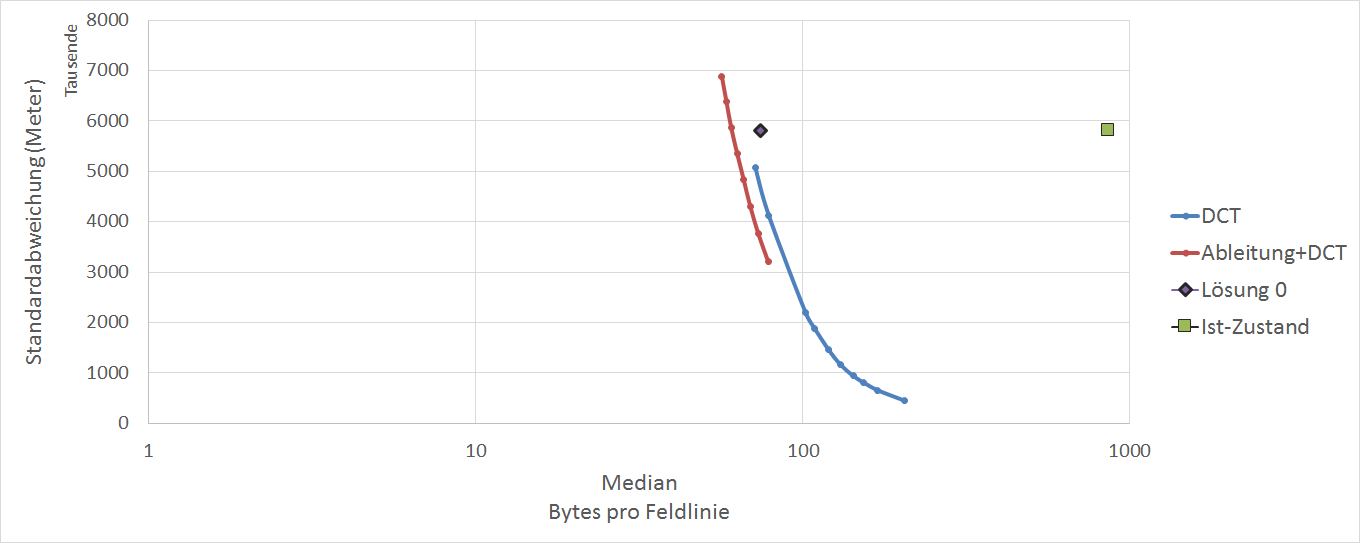
\includegraphics[width=1\textwidth,keepaspectratio]{./pictures/resultate/loesung1/loesung1-1/loesung1_1.png}
	\caption{Vergleich der DCT Kompression der Ableitung mit der DCT Kompression}
	\label{resultate:loesung1:dct_ableitung:resultate}
\end{figure}
Das Diagramm der Abbildung \ref{resultate:loesung1:dct_ableitung:resultate} zeigt, dass die abgeleiteten Feldlinien besser approximiert werden können als die vorhergehende Variante. Bei einer vergleichbaren Genauigkeit wie der Ist-Zustand erreicht diese Variante eine Kompressionsrate von $14.3$. Eine Darstellung der Artefakte ist im Diagramm der Abbildung \ref{resultate:loesung1:dct:byte:artefakte} zu finden. Die Artefakte der Kompression äussern sich als Dämpfungen. Die Artefakte sind jedoch für das menschliche Auge nicht sichtbar. Die Dämpfung ist erst zu erkennen, wenn das Original zur Verfügung steht.

\begin{figure}[!htbp]
	\center
	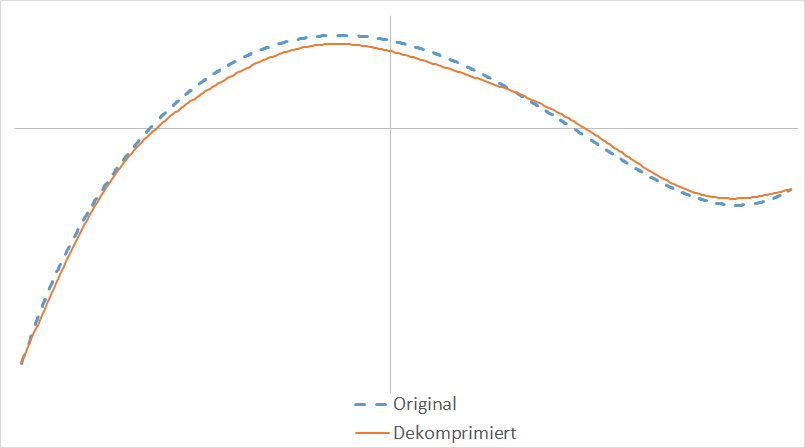
\includegraphics[width=0.8\textwidth,height=8cm,keepaspectratio]{./pictures/resultate/loesung1/loesung1-6/artefakte.png}
	\caption{Artefakte der DCT Kompression der Ableitung}
	\label{resultate:loesung1:dct:byte:artefakte}
\end{figure} 

\subsubsection{Variante: PCA+Ableitung+DCT}
Die Feldlinien dehnen sich nicht in alle Richtungen gleich stark aus: Es existieren Feldlinien, welche beinahe in einer Ebene liegen im dreidimensionalen Raum. Durch eine Principal Component Analysis (PCA)\cite{abdi2010principal} können die Feldlinien in ein lokales Koordinatensystem transformiert werden, in welchem die Kanäle unterschiedlich stark quantisiert werden können. Für die Rücktransformation ins Sonnen-Koordinatensystem werden pro Feldlinie zusätzlich sechs Parameter für die neuen Koordinatenachsen und drei Parameter für die Verschiebung abgespeichert.

\begin{figure}[!htbp]
	\center
	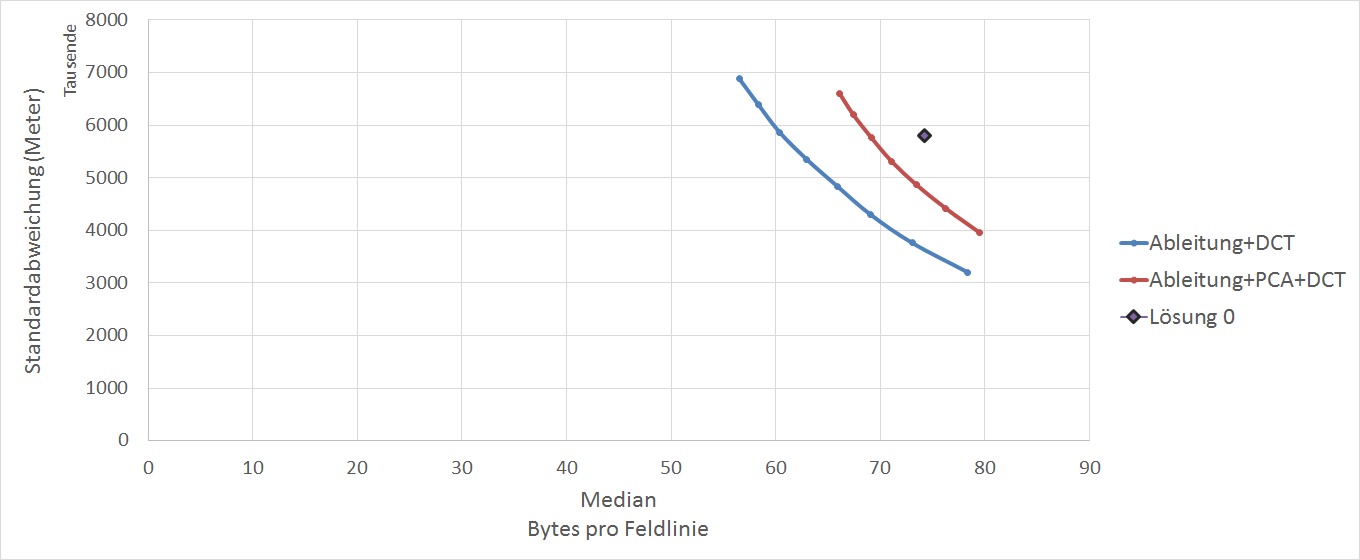
\includegraphics[width=1\textwidth,keepaspectratio]{./pictures/resultate/loesung1/loesung1-4/loesung1_4.png}
	\caption{Vergleich der PCA DCT Kompression der Ableitung mit der DCT Kompression der Ableitung}
	\label{resultate:loesung1:dct:pca}
\end{figure}
Im Diagramm der Abbildung \ref{resultate:loesung1:dct:pca} sind die Resultate der Messung dargestellt. Die PCA konnte keine Verbesserung erbringen. Für die Übermittlung der zusätzlichen Parameter wird mehr Speicherplatz benötigt, als dank der PCA gewonnen werden kann.

\subsubsection{Variante: Ableitung+DCT+Kodierung} \label{resultate:loesung1:ableitung_dct_kodierung}
Im Diagramm der Abbildung \ref{resultate:loesung1:dct:histogramm} ist zu sehen, dass der Grossteil der quantisierten DCT-Koeffizienten mit 8 Bit Genauigkeit dargestellt werden können. Um die Kompressionsrate durch diese Eigenschaft zu verbessern, wurde die Längenkodierung und die adaptive Kodierung entwickelt, welche im Abschnitt \ref{konzept:loesung1:kodierung} beschrieben sind.
\begin{figure}[!htbp]
	\center
	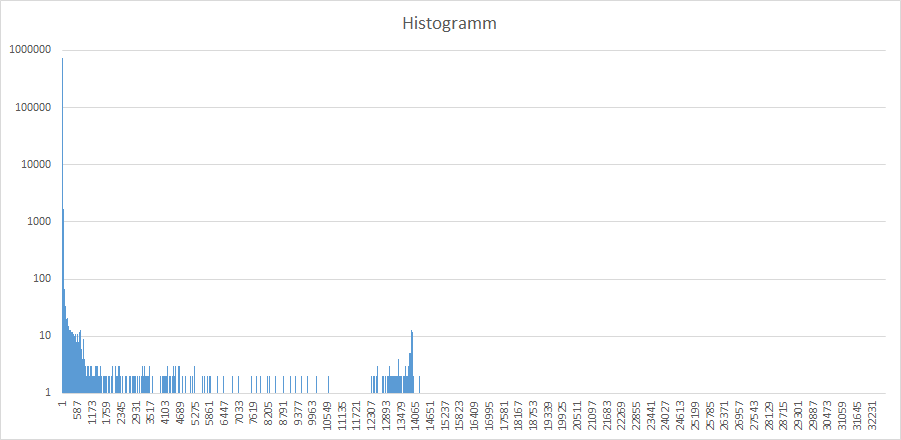
\includegraphics[width=1\textwidth,keepaspectratio]{./pictures/resultate/loesung1/loesung1-6/histo.png}
	\caption{Histogramm der absoluten Werte der 16 Bit DCT-Koeffizienten.}
	\label{resultate:loesung1:dct:histogramm}
\end{figure}

\begin{figure}[!htbp]
	\center
	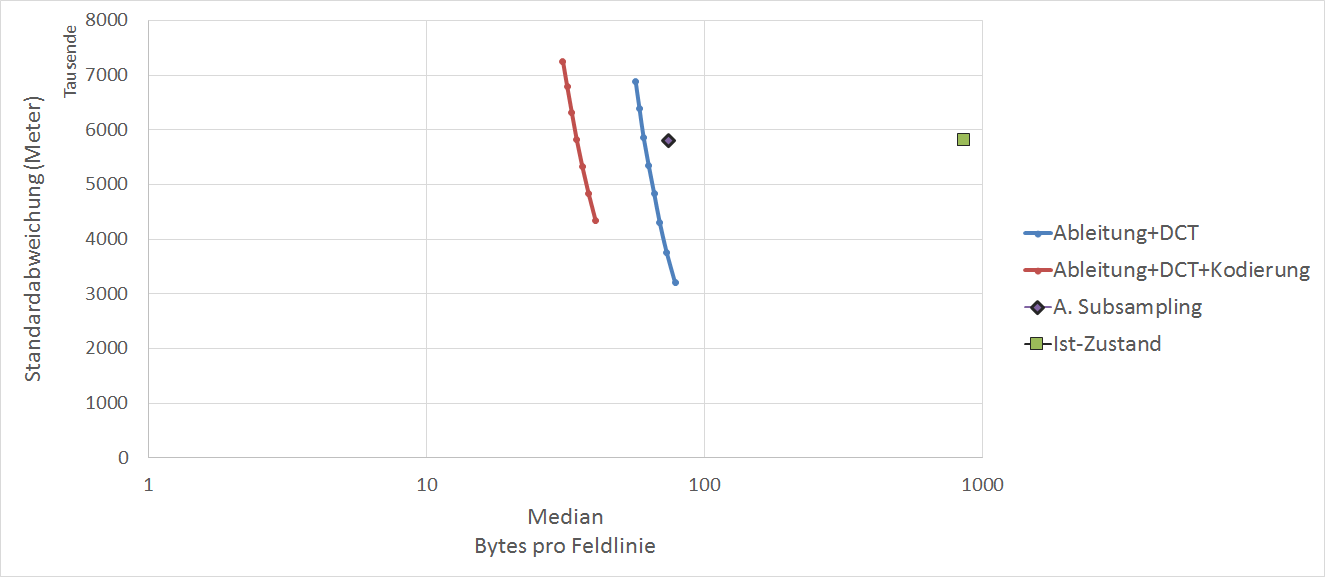
\includegraphics[width=1\textwidth,keepaspectratio]{./pictures/resultate/loesung1/loesung1-6/loesung1_6.png}
	\caption{Vergleich der Kompression mit und ohne Kodierung}
	\label{resultate:loesung1:dct:kodierung}
\end{figure}
Das Diagramm der Abbildung \ref{resultate:loesung1:dct:kodierung} zeigt den Einfluss der Kodierung auf die Kompressionsrate. Es bewirkt eine deutliche Verbesserung gegenüber der vorhergehenden Variante, ohne die Qualität der Kompression negativ zu beeinflussen. Bei einer Vergleichbaren Genauigkeit wie die Ist-Kompression weist diese Variante eine Kompressionsrate von $24.5$ auf.

\subsubsection{Variante: Randbehandlung+DCT+Kodierung} \label{resultate:loesung1:dct:randbeh+byte}
Bei dieser Variante wird mit zusätzlichen Daten am Anfang und am Ende der Feldlinie die Artefakte aus Abschnitt \ref{resultate:dct} behoben. Die Zusätzlichen Daten lassen die Feldlinie abflachen. Es wird erforscht, ob diese Darstellung der Feldlinien eine bessere Kompressionsrate zur ähnlichen Abweichung erlaubt. 

\begin{figure}[!htbp]
	\center	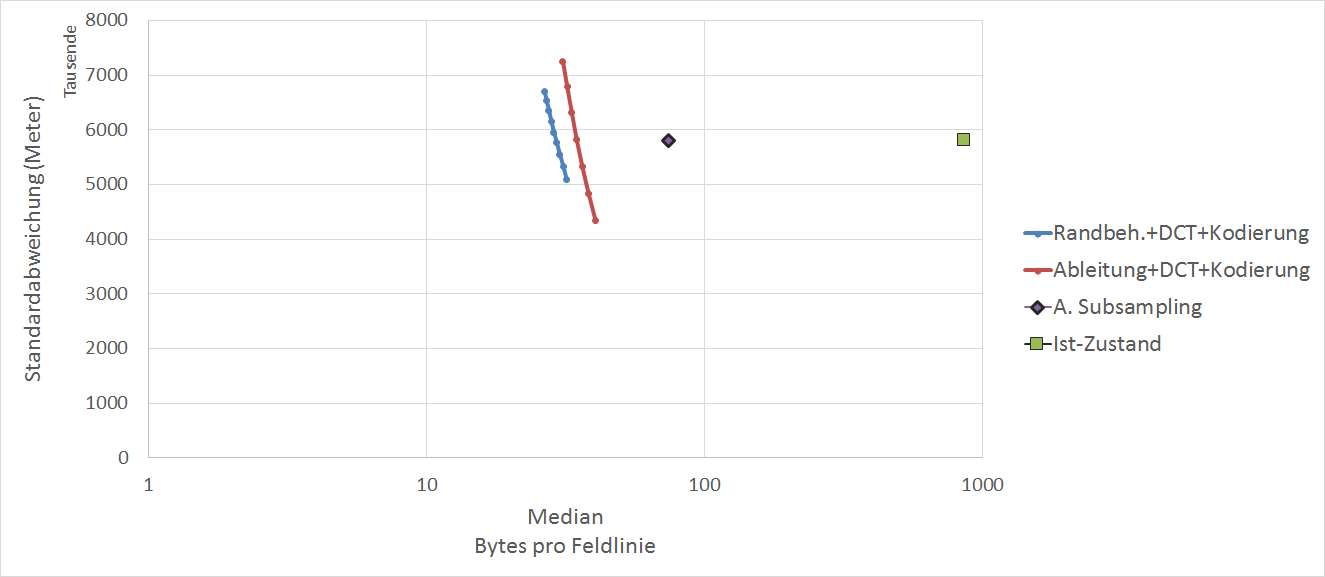
\includegraphics[width=1\textwidth,keepaspectratio]{./pictures/resultate/loesung1/loesung1-7/loesung1_7.png}
	\caption{Vergleich des Einflusses der Randbehandlung}
	\label{resultate:loesung1:dct:randbehandlung}
\end{figure}
Das Diagramm der Abbildung \ref{resultate:loesung1:dct:randbehandlung} zeigt den Vergleich der Variante mit Randbehandlung und der vorgehenden Variante, welche die Feldlinie ableitet. Die zusätzlichen Daten erlauben eine höhere Kompressionsrate zu einer ähnlichen Abweichung.\\
Diese Variante führt Artefakte ein, welche in der Standardabweichung nicht ins Gewicht fallen. Im folgenden Abschnitt \ref{resultate:loesung1:ringing} werden diese Artefakte besprochen.

\subsubsection{Ringing-Artefakte}\label{resultate:loesung1:ringing}
Obwhol die Variante aus Abschnitt \ref{resultate:loesung1:dct:randbeh+byte} eine vergleichbare Standardabweichung aufweist, wie die Ist-Kompression, sind auf der JHelioviewer Visualisierung deutliche Artefakte zu sehen. Die Abbildung \ref{resultate:loesung1:dct:randbehandlung:jvhartefakte} vergleicht die originalen mit dekomprimierten Feldlinien. Die Artefakte äussern sich als Oszillationen in den dekomprimierten Feldlinien.

\begin{figure}[!htbp]
	\center
	\frame{
	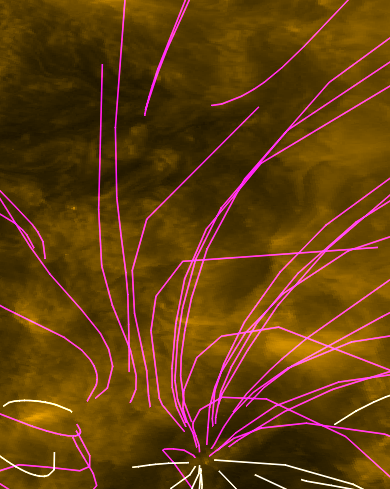
\includegraphics[width=0.8\textwidth,height=6cm,keepaspectratio]{./pictures/resultate/loesung1/ringing/actual.png}}
		\frame{
	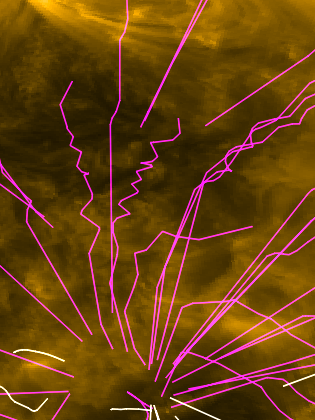
\includegraphics[width=0.8\textwidth,height=6cm,keepaspectratio]{./pictures/resultate/loesung1/ringing/sol7.png}}
	\caption{Artefakte der Kompression. Links sind die originalen Feldlinien, rechts die Dekomprimierten.}
	\label{resultate:loesung1:dct:randbehandlung:jvhartefakte}
\end{figure} 
In diesem Fall scheint die Standardabweichung als Fehlermass zu versagen: Da die Oszillationen nahe an der originalen Feldlinie liegen, bleiben die Abweichung klein. Jedoch sind die Artefakte für das menschliche Auge inakzeptabel.\\
Interessant ist, dass die abgeleiteten Feldlinien aus Abschnitt \ref{resultate:loesung1:ableitung_dct_kodierung} ähnliche Artefakte aufweisen, jedoch sind sie weniger ausgeprägt. Die Ableitung scheint die Artefakte zu dämpfen. Die Abbildung \ref{resultate:loesung1:dct:randbehandlung:jvhartefakte_loesung6} zeigt die Artefakte der abgeleiteten Feldlinien.

\begin{figure}[!htbp]
	\center
	\frame{
	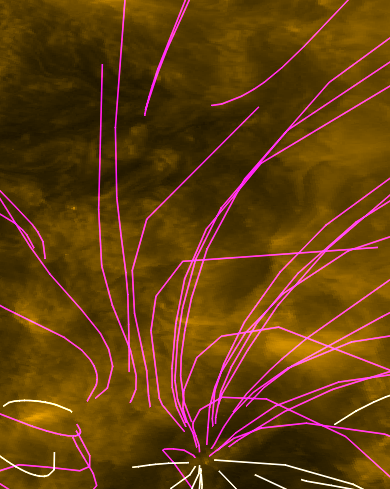
\includegraphics[width=0.8\textwidth,height=6cm,keepaspectratio]{./pictures/resultate/loesung1/ringing/actual.png}}
		\frame{
	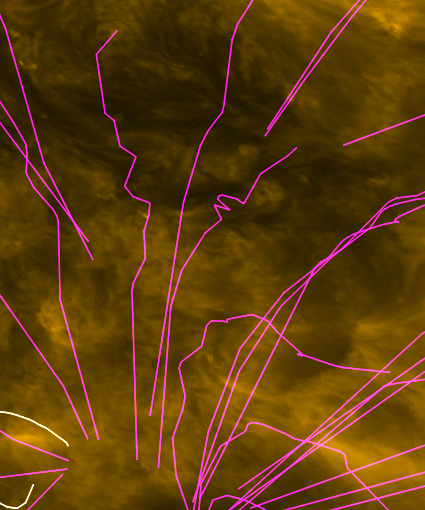
\includegraphics[width=0.8\textwidth,height=6cm,keepaspectratio]{./pictures/resultate/loesung1/ringing/sol6.png}}
	\caption{Artefakte der Kompression, links sind die originalen Feldlinien, rechts die Dekomprimierten der Variante \ref{resultate:loesung1:ableitung_dct_kodierung}.}
	\label{resultate:loesung1:dct:randbehandlung:jvhartefakte_loesung6}
\end{figure}
Die oszillierenden Artefakte sind typisch für eine Datenkompression mit einer Diskreten Kosinus Transformation und sind als Ringing-Artefakte \cite{wiki:ringing:artefacts} bekannt. Sie treten ebenfalls bei JPEG/JFIF oder MP3 Kompressionen auf: Abrupte Steigungen im Inputsignal werden in der DCT durch hochfrequente Anteile dargestellt. Durch die Quantisierung der hochfrequenten Anteile werden oszillierende Artefakte eingefügt.\\
Die Feldlinien, welche am stärksten von den Artefakten betroffen sind, sind die ''Weltall zur Sonne'' oder ''Sonne ins Weltall'' Feldlinien. Sie verhalten sich nicht wie harmonische Halbwellen sondern steigen oft monoton, mit teils abrupten Richtungswechseln in der Nähe der Sonnenoberfläche. Die Abbildung \ref{resultate:loesung1:dct:randbehandlung:harte_richtungswechsel} zeigt ein Beispiel solcher Feldlinien. Die abrupten Wechsel führen zu abrupten Steigungen in den einzelnen Kanälen.

\begin{figure}[!htbp]
\center
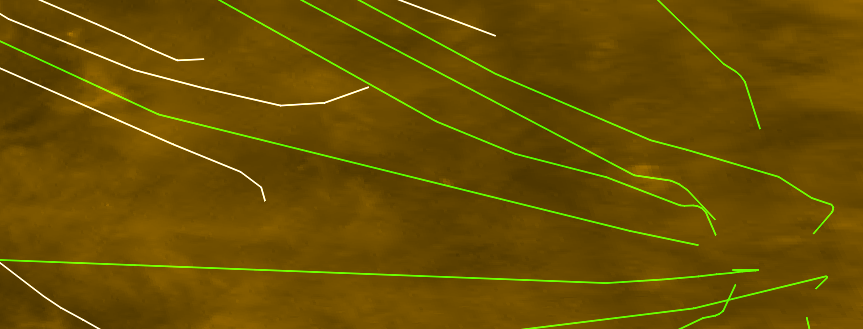
\includegraphics[width=0.4\textwidth,height=6cm,keepaspectratio]{./pictures/resultate/loesung1/ringing/haar-like.png}
	\caption{Abrupte Steigungen bei Feldlinien, welche von der Sonne ins Weltall führen.}
	\label{resultate:loesung1:dct:randbehandlung:harte_richtungswechsel}
\end{figure}

\subsubsection{Behandlung der Ringing-Artefakte} \label{resultate:loesung1:behandlung_ringing}
Um eine optimale Kompression der Feldlinien zu erreichen, müssen die Ringing-Artefakte behandelt werden. Im Abschnitt \ref{resultate:loesung1:ringing} wurde erwähnt, dass nicht alle Varianten gleich ausgeprägte Artefakte verursachen. Es wurde ebenfalls besprochen, dass die Feldlinien, welche von der Sonnenoberfläche zu Oberfläche führen, weniger ausgeprägte Artefakte mit sich bringen. In diesem Abschnitt wird erforscht, welche Variante die ''Sonne zu Sonne'' und welche die ''Weltall zur Sonne'' oder ''Sonne ins Weltall'' Feldlinien optimal approximieren kann, ohne zusätzliche Ringing-Artefakte hinzuzufügen. Für die Messung der Artefakte wird die PSNR-HVS-M Metrik aus Abschnitt \ref{testsetup:psnr} verwendet.\\
Für den Test werden insgesamt vier Varianten verglichen. Die Variante der abgeleiteten Feldlinien aus Abschnitt \ref{resultate:loesung1:ableitung_dct_kodierung} und die Variante der Randbehandlung aus Abschnitt \ref{resultate:loesung1:dct:randbeh+byte}. Die Varianten werden jeweils mit und ohne einer PCA gemessen. Die PCA wird hier nochmals überprüft, da sie die Ringing-Artefakte auf einen Kanal beschränken kann.

\begin{figure}[!htbp]
	\center	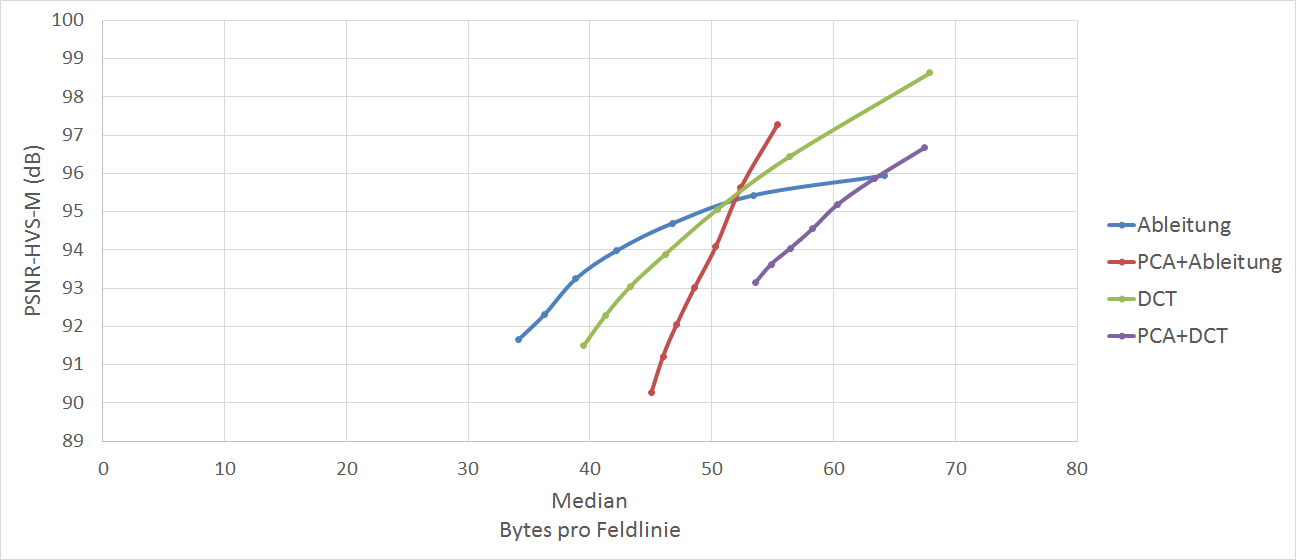
\includegraphics[width=1\textwidth,keepaspectratio]{./pictures/resultate/loesung1/ringing/sts.png}
	\caption{Approximation der Feldlinien ''Sonnenoberfläche zu Sonnenoberfläche''. Je höher die PSNR-HVS-M, desto besser ist die Approximation. }	\label{resultate:loesung1:dct:behandlung_ringing:sts}
\end{figure} 
\begin{figure}[!htbp]
	\center
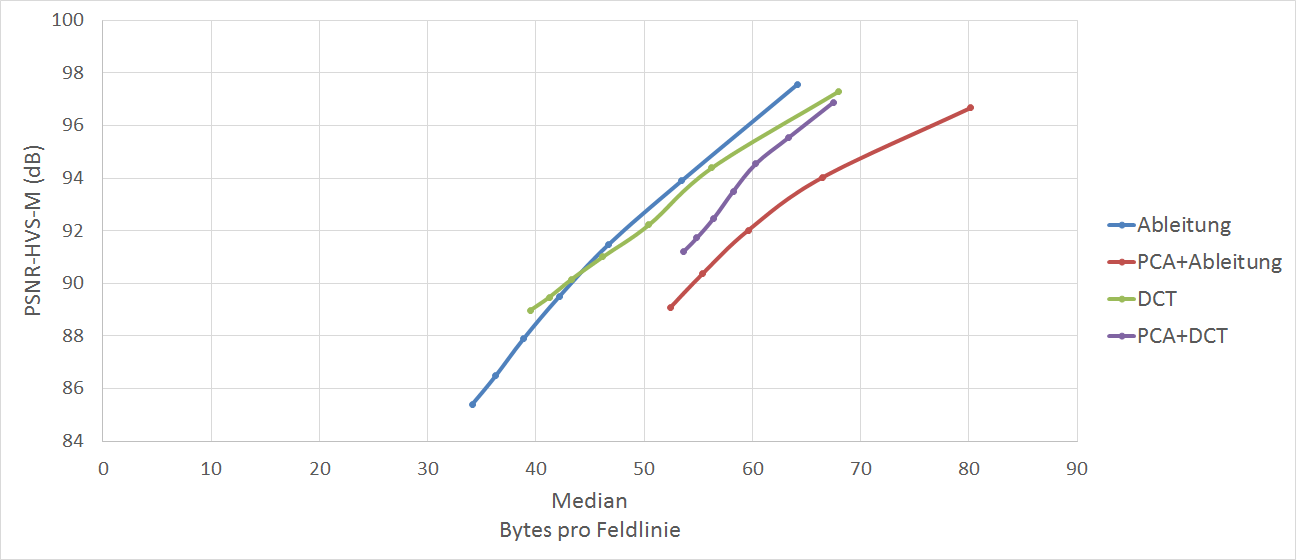
\includegraphics[width=1\textwidth,keepaspectratio]{./pictures/resultate/loesung1/ringing/nosts.png}
	\caption{Approximation der der Feldlinien ''Sonnenoberfläche ins Weltall'' oder ''Weltall zur Sonnenoberfläche''. Je höher die PSNR-HVS-M, desto besser ist die Approximation.}	\label{resultate:loesung1:dct:behandlung_ringing:nosts}
\end{figure}
Das Diagramm der Abbildung \ref{resultate:loesung1:dct:behandlung_ringing:sts} zeigt die Resultate der unterschiedlichen Varianten bei den Feldlinien ''Sonnenoberfläche zur Sonnenoberfläche''. Bei einer PSNR-HVS-M von über $95$ dB sind die Artefakte genügend schwach ausgeprägt, sodass das menschliche Auge sie nicht mehr erkennen kann. Interessant ist, dass drei Varianten ähnlich viel Speicherplatz benötigen, für eine artefaktfreie Approximation. Bei stärkerer Quantisierung treten bei den abgeleiteten Feldlinien deutlich weniger Artefakte auf. Dies deckt sich mit der Beobachtung aus dem Abschnitt \ref{resultate:loesung1:ringing}.\\
Ebenfalls interessant ist die Variante der PCA Transformation zusammen mit der Ableitung: Diese benötigt für eine beinahe artefaktfreie Approximation am wenigsten Speicherplatz, führt aber bei stärkerer Quantisierung viele Artefakte ein.

Das Diagramm der Abbildung  \ref{resultate:loesung1:dct:behandlung_ringing:nosts} zeigt, wie gut die Varianten die Feldlinien ''Sonne ins Weltall'' und ''Weltall zur Sonne'' approximieren können. Bei diesen Typen von Feldlinien dämpft die Ableitung ebenfalls die Artefakte. Jedoch weniger deutlich als bei den ''Sonne zur Sonne'' Feldlinien. Die PCA konnte auch bei diesen Typen von Feldlinien keinen messbaren Vorteil erbringen. Die zusätzlichen Parameter der PCA verbrauchen mehr Speicherplatz als durch die Transformation gewonnen werden.\\
Die DCT Variante aus Abschnitt \ref{resultate:loesung1:dct:randbeh+byte} fällt ab einer PSNR-HVS-M von $90 dB$ weniger schnell ab als die abgeleiteten Feldlinien. Bei diesem PSNR-HVS-M Wert sind aber die Artefakte bereits zu deutlich und nicht mehr akzeptabel. Aufgrund dieser Resultate wurde die Variante der abgeleiteten Feldlinien von Abschnitt \ref{resultate:loesung1:ableitung_dct_kodierung} ausgewählt. 

\subsubsection{Abschliessende Variante}
Für den abschliessenden Tests wurde die Variante der abgeleiteten Feldlinien aus Abschnitt \ref{resultate:loesung1:ableitung_dct_kodierung} ausgewählt. Durch die Ableitung können die Ringing-Artefakte gedämpft werden. Die Quantisierung wurde angepasst, sodass die Feldlinien vom Typ ''Sonne zu Sonne'' stärker quantisiert werden, als die anderen Feldlinien. Durch diese Massnahme wird eine hohe Kompressionsrate erreicht ohne starke Ringing-Artefakte mit sich zu ziehen.

\begin{figure}[!htbp]
	\center	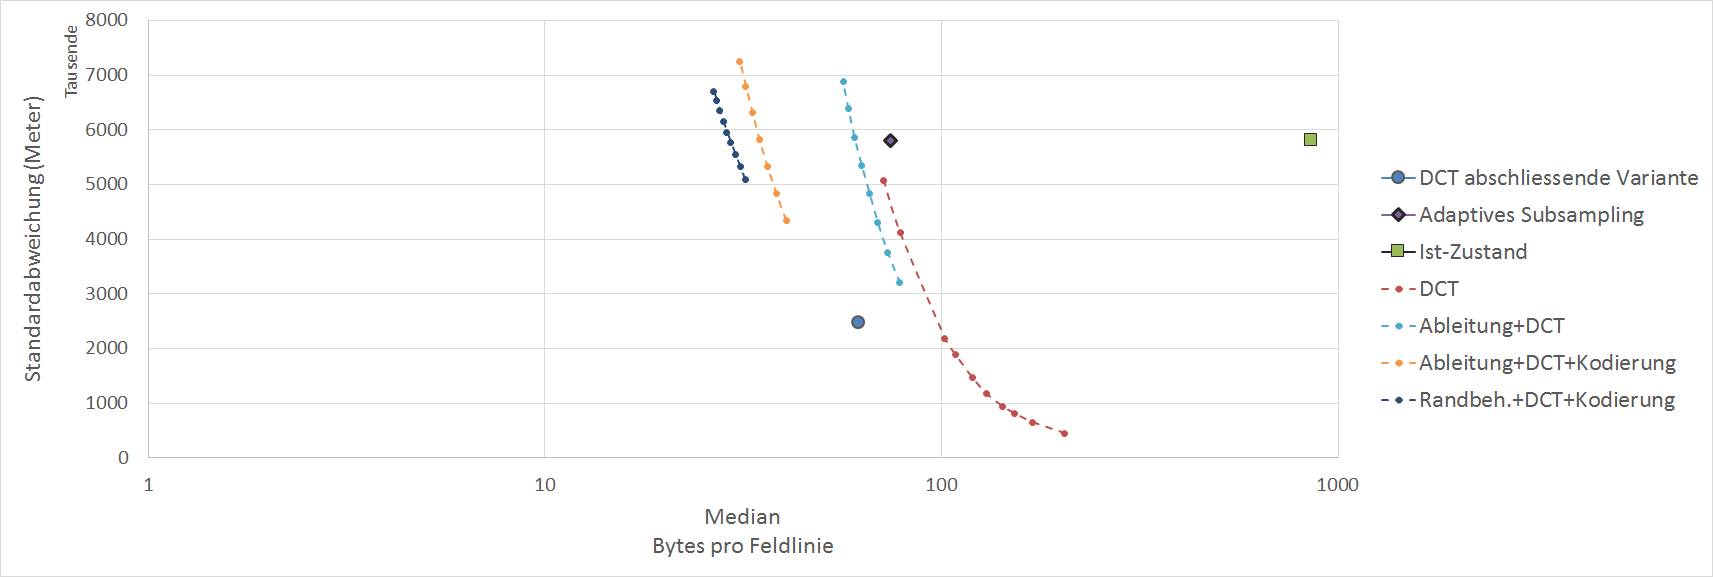
\includegraphics[width=1\textwidth,keepaspectratio]{./pictures/resultate/loesung1/loesung1-12/resultate.png}
	\caption{Standardabweichung der abschliessenden DCT Variante.}	\label{resultate:loesung1:dct:abschliessend:standardabweichung}
\end{figure} 
Das Diagramm der Abbildung \ref{resultate:loesung1:dct:abschliessend:standardabweichung} zeigt die Standardabweichung der abschliessenden DCT Variante. Sie erreicht eine höhere Kompression als das Verfahren des Adaptiven Subsamplings und kann die Feldlinie zu einer tieferen Standardabweichung approximieren. Es wurde eine durchschnittliche Kompressionsrate $14.1$ erreicht, obwohl eine höhere Anzahl an Werte übertragen wird. Die Problematik dieses Verfahrens liegt darin, dass die DCT Kompression Ringing-Artefakte hinzufügt.\\
Durch die unterschiedliche Quantisierungen konnten die Ringing-Artefakte in Grenzen gehalten werden und erreichen einen PSNR-HVS-M  Wert von $94.0$. Die ''Sonne zu Sonne'' Feldlinien können deutlich besser approximiert werden als die anderen Feldlinien. Würde die Simulation nur aus diesen Feldlinien bestehen, könnte eine Kompressionsrate von $15-18$ erreicht werden zu einem ähnlichen PSNR-HVS-M Wert. Die Feldlinien ''Sonne ins Weltall und ''Weltall zur Sonne'' sind schwieriger mit einer DCT artefaktfrei zu approximieren.  Durch das Zoom Feature vom JHelioviewer ist der Benutzer in der Lage die Ringing-Artefakte zu finden, sobald sie existieren. Das Linke Bild der Abbildung \ref{resultate:loesung1:dct:final:artefakte} zeigt die Artefakte der Kompression. Die Artefakte sind aus der Simulation, welche die markantesten Ringing-Artefakte aufweist.

\begin{figure}[!htbp]
	\center
	\frame{
	
\includegraphics[width=0.8\textwidth,height=5cm,keepaspectratio]{./pictures/resultate/loesung1/loesung1-12/without_average_line.png}}
		\frame{
	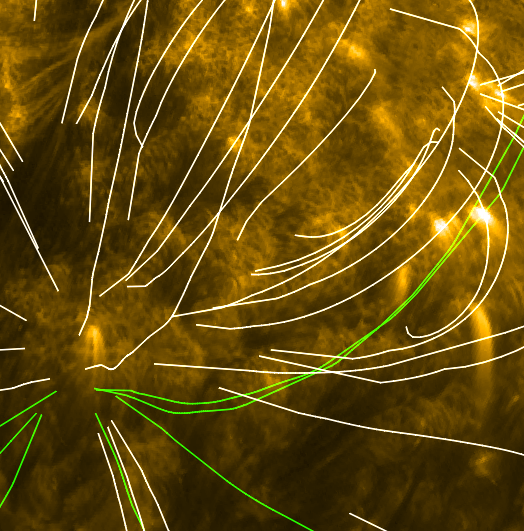
\includegraphics[width=0.8\textwidth,height=5cm,keepaspectratio]{./pictures/resultate/loesung1/loesung1-12/with_average_line.png}}
	\caption{Die am stärksten ausgeprägten Artefakte der abschliessenden Variante. Links ohne Glättung, rechts mit Glättung}
	\label{resultate:loesung1:dct:final:artefakte}
\end{figure}
Durch eine Kurvenglättung kann der JHelioviewer die Artefakte verschleiern. Die komprimierten Daten enthalten mehr Werte, als die JHelioviewer Visualisierung darstellen kann. Die zusätzlichen Werte werden zur Glättung der Feldlinie verwendet. Den Effekt der Glättung ist in der Abbildung \ref{resultate:loesung1:dct:final:artefakte} abgebildet.\\
Im Abschnitt \ref{konzept:loesung1} wurde erwähnt, dass Reduktion von Ringing-Artefakte ein aktives Forschungsfeld der Bildverarbeitung ist. Es existieren Post-Processing Filter, welche Ringing-Artefakte von dekomprimierten Bildern vermindern. Eine Möglichkeit die Kompression zu verbessern ist es, einen Post-Processing Filter für wissenschaftliche Daten zu entwickeln. Eine weitere Möglichkeit ist die Diskrete Kosinus Transformation durch eine Wavelet Transformation zu ersetzen. Diese ist weniger anfällig auf Ringing-Artefakte und hat das Potential eine ähnlich gute Kompression zu erreichen.

Beim Caching von $1000$ Simulationen benötigt dieser Ansatz $70$ Megabyte Arbeitsspeicher, etwa $15$ Megabyte weniger als das Verfahren des Adaptiven Subsamplings. Wenn von derselben $5$ Megabit Internenetverbindung ausgegangen wird, werden $112$ Sekunden benötigt um $1000$ Simulationen herunterzuladen. Pro Sekunde werden $9$ anstatt $7$ Simulationen übertragen.

Die höhere Kompressionsrate führt zu einer höheren Komplexität der Dekompression. Die Laufzeit der Dekompression hängt im Wesentlichen von der Implementation der inversen DCT ab. Eine naive Implementation braucht für eine Dekompression etwa drei Sekunden (siehe Abschnitt \ref{anhang:performance}. Die grösste Zeit wird in der Berechnung der Kosinus-Werte verbraucht. Bei der DCT Implementation in dieser Arbeit werden die Kosinus-Werte über SoftReferences gecached. Der Cache passt sich somit an den Arbeitsspeicher an. Wie schnell die Dekompression ist, hängt im Wesentlichen vom verfügbaren Arbeitsspeicher ab. Im besten Fall ergibt das eine Laufzeit von $65$ Millisekunden und im schlechtesten Fall $350$. Mit einer Java Implementation der Fast-Cosine-Transform wird eine Laufzeit von $100$ bis $135$ Millisekunden erreicht. Im besten Fall ist die Implementation für diese Arbeit schneller, da es die Eigenschaft der Quantisierung ausnutzen kann: Es werden pro Feldlinie maximal $50$ Koeffizienten übertragen. Die Komplexität kann dadurch auf $O(n*m)$ beschränkt werden, wobei $m$ die Anzahl der Koeffizienten ist. Die FDCT weist eine Komplexität von $O(n log(n))$ auf. Die Implementation verliert Laufzeit gegenüber der FDCT, wenn die Kosinus-Koeffizienten neu berechnet werden. Im Durchschnittsfall ist die FDCT Implementation schneller, was einen Durchsatz von $8$ Simulationen pro Sekunde pro Thread führt.\\

\pagebreak
\subsection{Lösungsansatz: Prediktive Kodierung}
In diesem Abschnitt wird der Lösungsansatz der Prädiktiven Kodierung besprochen. Es wurde der Einfluss von verschiedenen Prädiktoren getestet. Die Schwierigkeit dieses Lösungsansatzes liegt in der Quantisierung des Vorhersagefehleres. Die Quantisierung der Fehler von einfacher Prädiktoren führt zu hohen Abweichungen in der Dekompression. Der Rekursive Lineare Prädiktor unter Abschnitt \ref{resultate:loesung2:wavelet} löst das Problem.

\subsubsection{Variante: einfaches Subsampling}
Für die erste Variante wird das Subsampling des DCT-Lösungsansatzes verwendet. Es reduziert die Punktmenge auf die Anzahl des Ist-Zustands. Die Feldlinien werden mit einer PCA in ein lokales Koordinatensystem transformiert. Im lokalen System können die Koordinaten mit 16 Bit Genauigkeit dargestellt werden. 16 Bit im Koordinatensystem der Sonne reichen nicht aus und führen zu einem grösseren Fehler als der Ist-Zustand.\\
In dieser Variante wird der Einfluss von vier Prediktoren getestet ($x$ sind die Bekannten Punkte und $y$ die Vorhersage):
\begin{itemize}
\item Konstanter Prediktor: Nimmt an, dass der nächste Wert im Kanal gleich dem  letzten Wert ist ($x = y$).
\item Linearer Prediktor: Nimmt an, dass die Steigung die Steigung zum nächsten Wert konstant bleibt ($x_1+(-x_2+x_1) = y$).
\item Linearer Prediktor mit Moving Average: Nimmt die durchschnittliche Steigung der letzten Werte.
\item Adaptiver Linearer Prediktor mit Moving Average: Berücksichtigt den Fehler der letzten Vorhersage.
\end{itemize}

\begin{figure}[!htbp]
	\center
	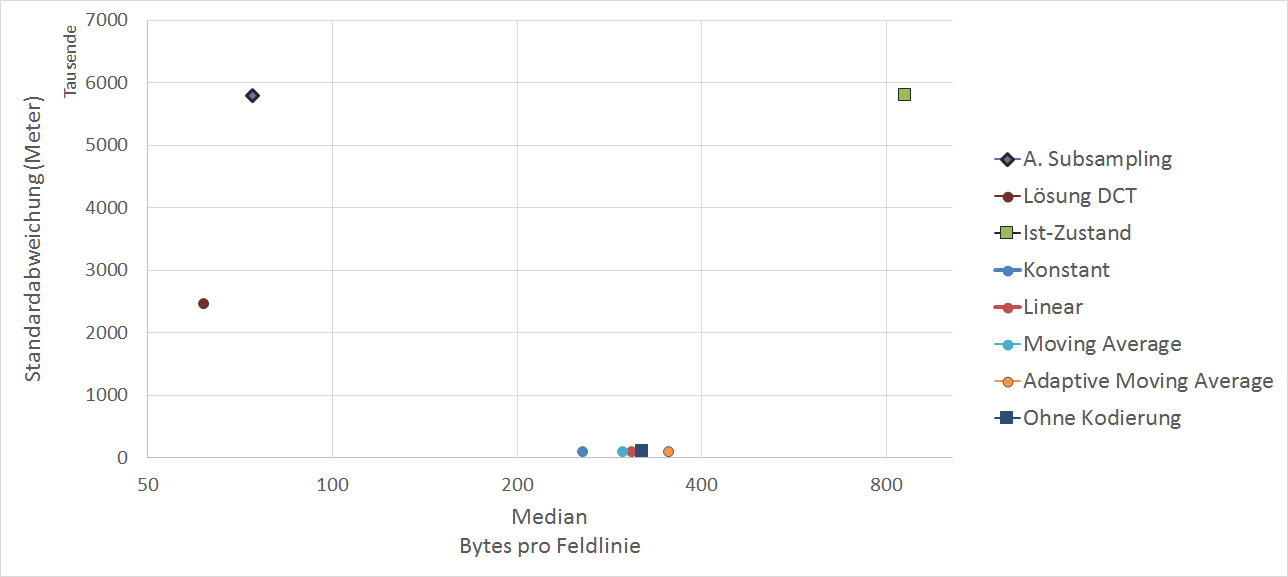
\includegraphics[width=1\textwidth,keepaspectratio]{./pictures/resultate/loesung2/variante0/resultate.png}
	\caption{Kompressionsraten der vier Prediktoren im Vergleich zum Ist-Zustand.}
	\label{resultate:loesung2:simple:resultate}
\end{figure}
Im Diagramm der Abbildung \ref{resultate:loesung2:simple:resultate} sind die Kompressionsraten der jeweiligen Prediktoren dargestellt. Ein Diagramm mit der PSNR-HVS-M wurde nicht erstellt. Sie ist für alle Prediktoren gleich und liegt bei $140.7$ dB. Unerwartet ist, dass der Konstante Prediktor mit $255$ Bytes pro Feldlinie die beste Kompression erreichte, obwohl die Daten nicht zuverlässig vorhersagen kann. Im Vergleich mit dem Moving Average Prediktor sind die Fehler der Vorhersagen 
bis zu $5$ Mal grösser, verbrauchen aber $40$ Bytes weniger um eine Feldlinie abzuspeichern. Der Fehler bleibt jedoch Konstant. Eine Möglichkeit ist, dass die Rar Kodierung sich wiederholende Muster findet.\\
Eine mögliche Optimierung ist die Adaptive Byte Kodierung der DCT-Variante, beschrieben im Abschnitt \ref{konzept:loesung1:kodierung}. Das Diagramm der Abbildung \ref{resultate:loesung2:simple:resultate_byte} zeigt die Resultate mit der Byte Kodierung. Der Konstante Prediktor verbraucht mit der Adaptiven Kodierung mehr Speicherplatz. Die Kompressionsrate der anderen Prediktoren wird durch die Adaptive Kodierung deutlich verbessert. Der Lineare Prediktor erreicht mit $214$ Bytes pro Feldlinie die beste Kompression. Das bedeutet, dass die Fehler des Konstanten Prediktors grösser sind, als die der anderen Prediktoren. Es bestätigt die Vermutung, dass die anderen Prediktoren die Daten besser vorhersagen können. Die Kompressionsrate des Konstanten Prediktors ist auf die Rar Kodierung zurückzuführen, welche in den Prediktor-Fehler Muster erkennen und effizient kodieren kann.\\ 
\begin{figure}[!htbp]
	\center
	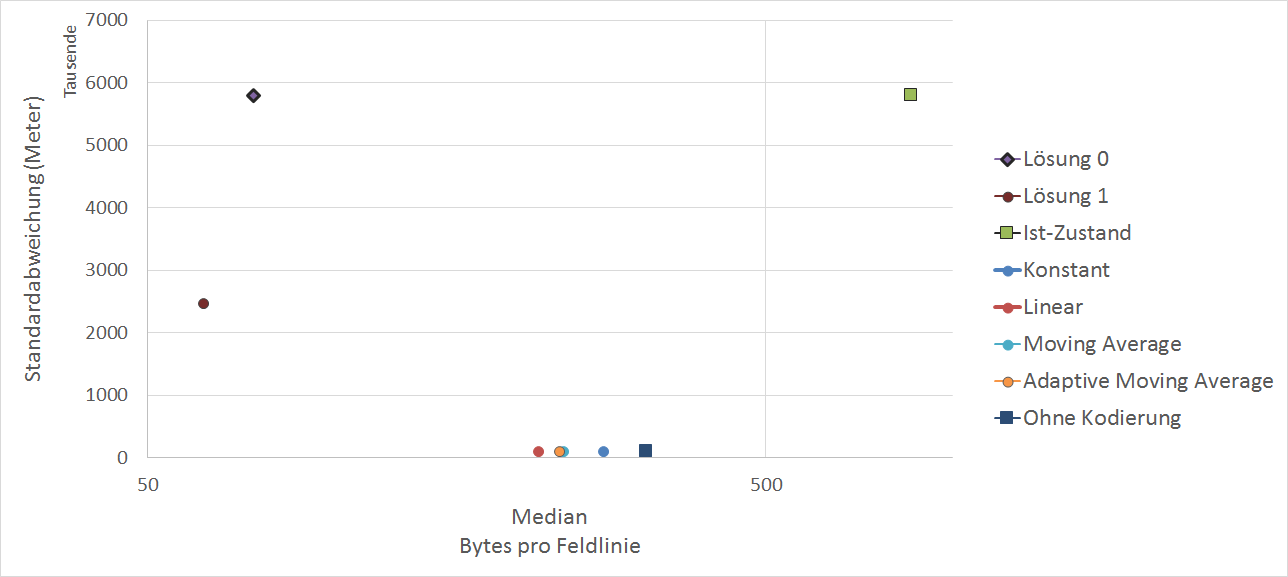
\includegraphics[width=1\textwidth,keepaspectratio]{./pictures/resultate/loesung2/variante0/resultate_byte.png}
	\caption{Kompressionsraten der Prediktoren mit Adaptiver Byte Kodierung.}
	\label{resultate:loesung2:simple:resultate_byte}
\end{figure}
Der Linare Prediktor kann eine Feldinie mit etwa $214$ Bytes darstellen, was eine Kompressionsrate von $4$ ergibt.

\subsubsection{Variante: Adaptives Subsampling}
Um mit diesem Ansatz in die selbe Grössenordnung zu gelangen wie die Lösungsansätze Adaptives Subsampling und DCT müssen mehr Informationen gelöscht werden. Es werden andere Parameter verwendet und im Schnitt $50\%$ mehr Punkte übertragen als im Lösungsansatz des Adaptiven Subsampling.\\
\begin{figure}[!htbp]
	\center
	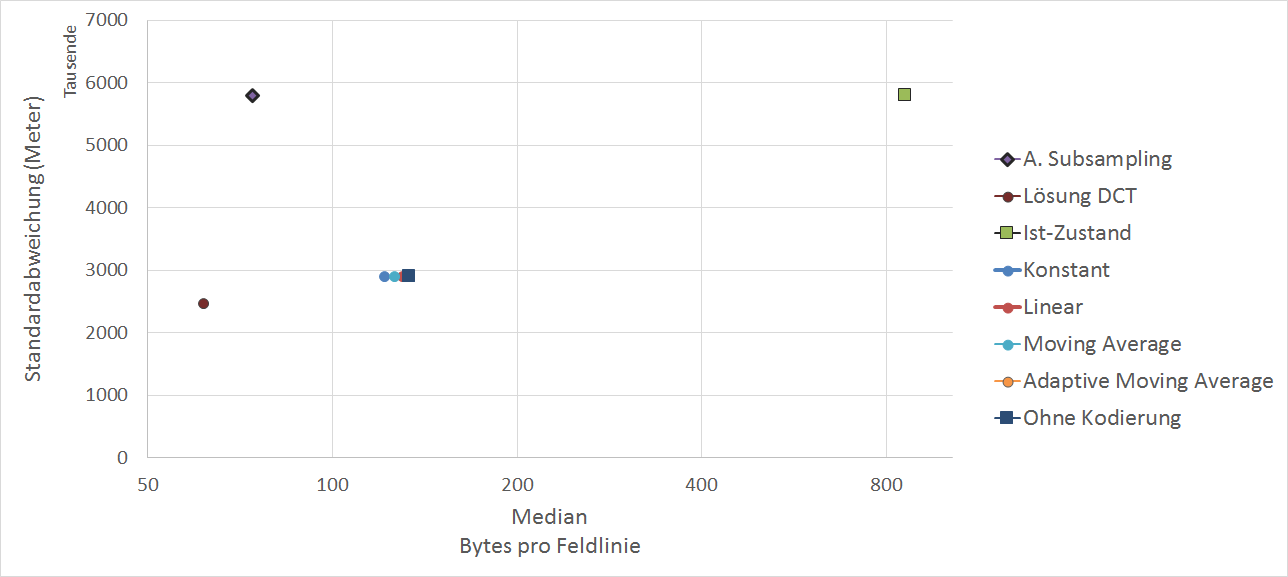
\includegraphics[width=1\textwidth,keepaspectratio]{./pictures/resultate/loesung2/variante1/resultate_euler.png}
	\caption{Kompressionsraten der Prediktiven Kodierungen mit dem adaptiven Subsampling.}
	\label{resultate:loesung2:adaptive:euler}
\end{figure}
Das Diagramm der Abbildung \ref{resultate:loesung2:adaptive:euler} zeigt die Kompressionsraten. Die Resultate liegen dicht beieinander und der Abstand zwischen Kodierung und der Kompression, welche ohne Kodierung erreicht wird wurde drastisch vermindert. Die Kodierungen erreichen eine PSNR-HVS-M von $139,2$. Das Angle Subsampling verändert die Eigenschaften der Daten. Die Diagramme der Abbildung \ref{resultate:loesung2:adaptive:channel} visualisiert die Veränderung. Monotone Steigungen sind nach dem Subsampling nicht mehr vorhanden. Die einfachen Prediktoren können die Daten nicht zuverlässig vorhersagen. 
\begin{figure}[!htbp]
	\center
	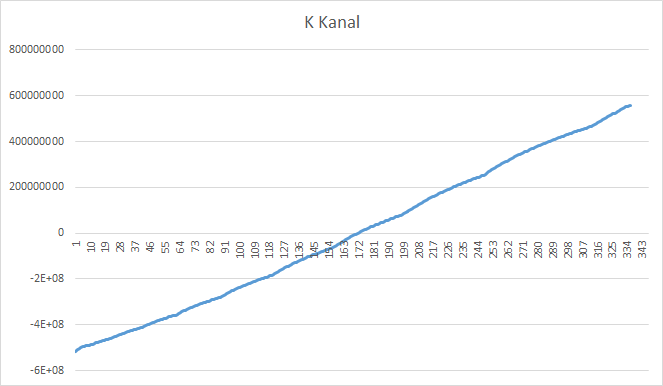
\includegraphics[width=0.49\textwidth,height=5cm,keepaspectratio]{./pictures/resultate/loesung2/variante1/channel_sub.png}
	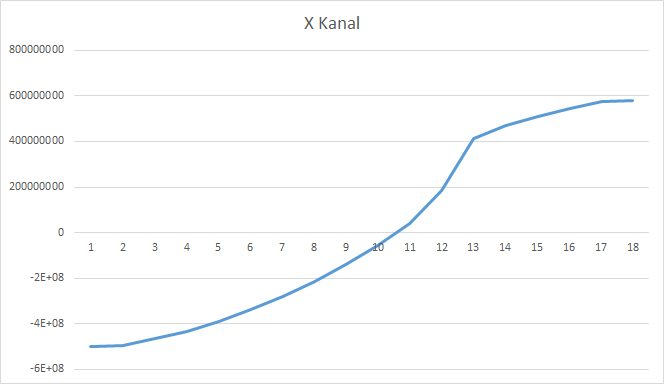
\includegraphics[width=0.49\textwidth,height=5cm,keepaspectratio]{./pictures/resultate/loesung2/variante1/channel_angle.png}
	\caption{Änderung der Eigenschaften der Daten durch das Angle Subsampling. Links der Kanal einer Feldlinie vor, rechts der Kanal nach dem Angle Subsampling.}
	\label{resultate:loesung2:adaptive:channel}
\end{figure}

\subsubsection{Rekursive Lineare Kodierung} \label{resultate:loesung2:wavelet}
Die Rekursive Lineare Kodierung ist in der Lage nicht-stetigen Kanälen eine sinnvolle Vorhersage zu berechnen. Das Verfahren ist im Abschnitt \ref{konzept:prediktiv} genauer erleutert. Die Punkte werden ins sphärische Koordinatensystem überführt. In diesem Koordinatensystem sind 16 Bit Genauigkeit pro Koordinatenachse ausreichend und die PCA muss nicht berechnet werden. Im Schnitt können dadurch $30$ Bytes pro Feldlinie eingespart werden. 
Zusätzlich werden die Vorhersagefehler quantisiert. Bei den einfachen Prediktoren wurde keine Quantisierung des Fehlers vorgenommen. Jede Quantisierung führte zu einem markanten Anstieg der Abweichung.\\
\begin{figure}[!htbp]
	\center
	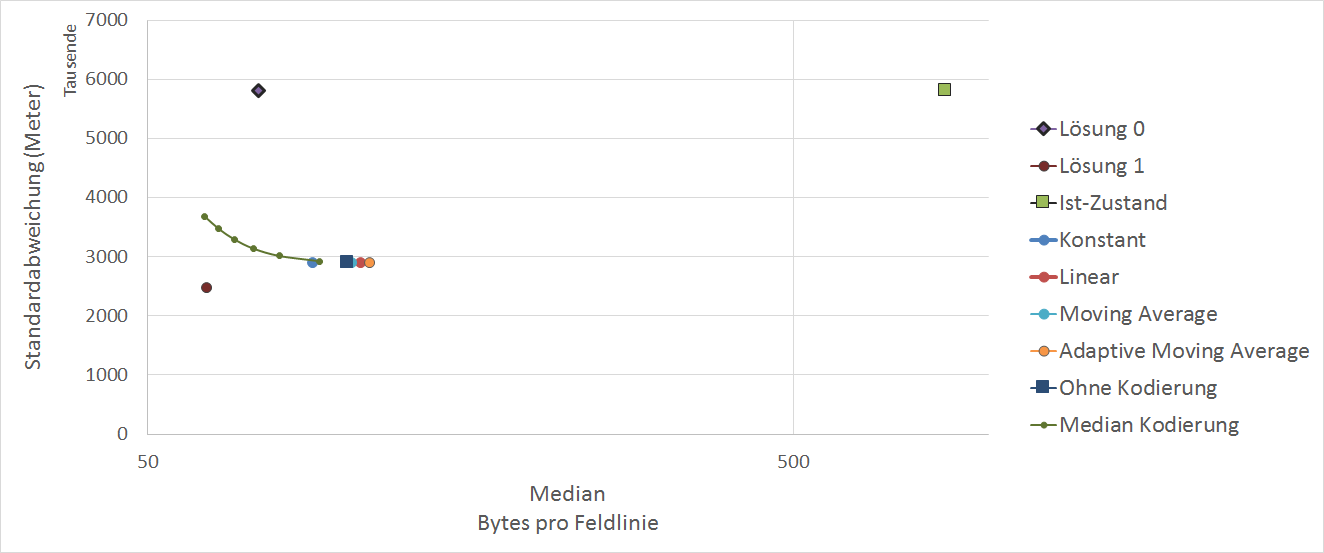
\includegraphics[width=1\textwidth,keepaspectratio]{./pictures/resultate/loesung2/variante2/resultate.png}
		\label{resultate:loesung2:adaptive:median}
		\caption{Kompressionsraten der Rekursive Lineare Kodierung mit dem adaptiven Subsampling.}
\end{figure}
\begin{figure}[!htbp]
	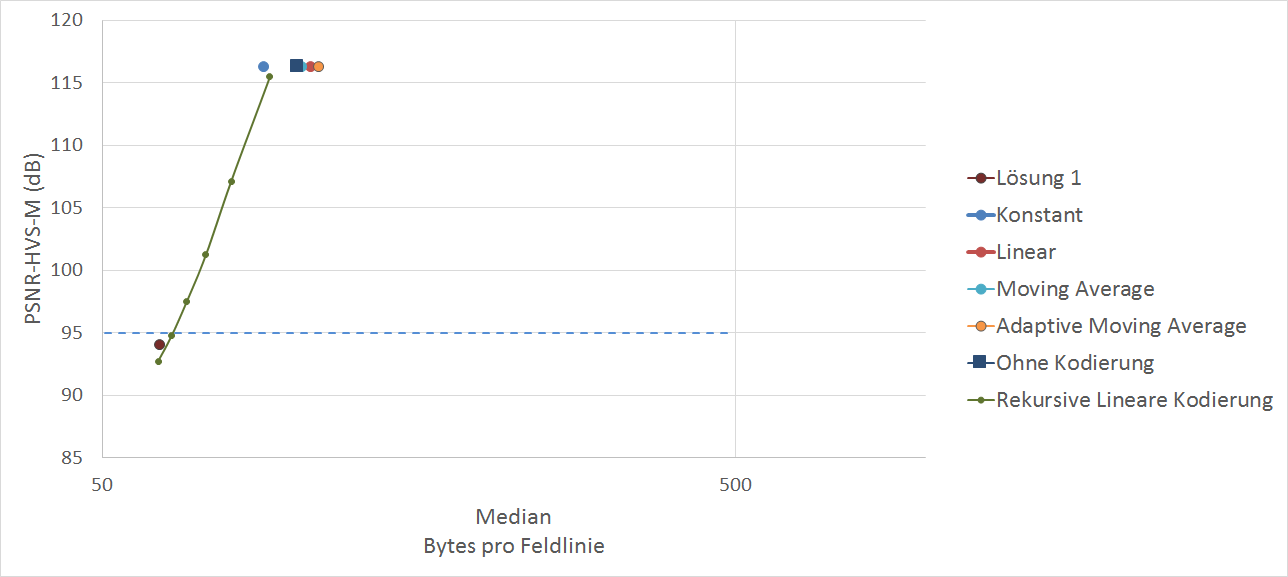
\includegraphics[width=1\textwidth,keepaspectratio]{./pictures/resultate/loesung2/variante2/resultate_psnr.png}
	\label{resultate:loesung2:adaptive:median_psnr}
	\caption{Kompressionsraten der Rekursive Lineare Kodierung mit dem adaptiven Subsampling.}
\end{figure}
Das Diagramm der Abbildung \ref{resultate:loesung2:adaptive:median} zeigt die Standardabweichung der Rekursiven Linearen Kodierung zu unterschiedlichen Quantisierungen. Das Diagramm der Abbildung \ref{resultate:loesung2:adaptive:median_psnr} zeigt die PSNR-HVS-M Werte der Variante. Die Resultate der einfachen Prediktoren wurden ebenfalls ohne PCA im sphärischen Koordinatensystem gemessen. Die Rekursive Lineare Kodierung kann eine bessere Kompressionsrate erreichen als die Lösung des Adaptiven Subsamplings. Bei Datenmenge von $64$ Bytes pro Feldlinie erreicht diese Variante eine tiefere Standardabweichung als das Adaptive Subsampling zu einem PSNR-HVS-M Wert von $94.7$. Dieser Ansatz besitzt weniger ausgeprägte Artefakte als die DCT Lösung, weist aber eine höhere Standardabweichung auf. Die Variante erreicht eine Kompressionsrate von $13.4$ und fällt somit zwischen den Lösungsansätzen DCT und Adaptives Subsampling.

Die Artefakte der Dekompression äussern sich meist als Verschiebungen einzelner Punkte. Im Extremfall können Ringing ähnlichen Artefakte entstehen, welche in der Abbildung \ref{resultate:loesung2:adaptive:median:artefakte} dargestellt sind. Die Artefakte sind weniger stark ausgeprägt als die des DCT Lösungsansatzes. Der Grund für die Artefaktbildung liegt in der Rekursion: Wenn der Vorhersagefehler des ersten Wertes (siehe Diagramm der Abbildung \ref{konzept:loesung2:algorithm:step1}) quantisiert wird, beeinflusst der Quantisierungsfehler den gesamten Kanal. Die Werte, welches als letztes Kodiert werden, erfahren die grösste Verschiebung bei der Dekompression. Diese Variante verwendet einen konstanten Faktor für die Quantisierung. Die Lösung ist eine angepasste Quantisierung, welche die ersten Vorhersagefehler mit höherer Genauigkeit abspeichert. 

\begin{figure}[!htbp]
	\center
		
\includegraphics[width=0.49\textwidth,height=5cm,keepaspectratio]{./pictures/resultate/loesung2/variante3/no_artifacts.png}
	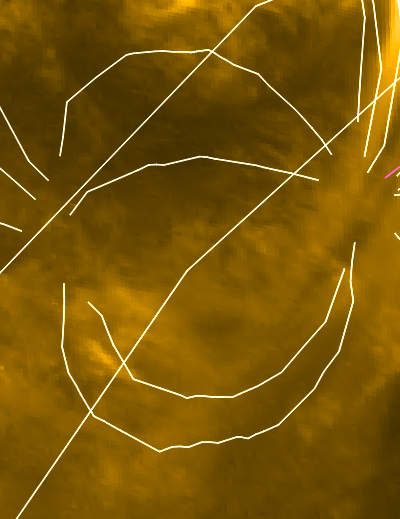
\includegraphics[width=0.49\textwidth,height=5cm,keepaspectratio]{./pictures/resultate/loesung2/variante3/artifacts_8.png}
	\caption{Artefakte der Rekursiven Linearen Kodierung. Links sind die originalen Feldlinien.}
	\label{resultate:loesung2:adaptive:median:artefakte}
\end{figure}

\subsubsection{Rekursive Lineare Kodierung mit angepasster Quantisierung}
Um die Artefakte der Dekompression zu dämpfen werden die Vorhersagefehler der Rekursionsstufe angepasst quantisiert. Die ersten Rekursionsstufen werden mit höherer Genauigkeit abgelegt.
\begin{figure}[!htbp]
	\center
	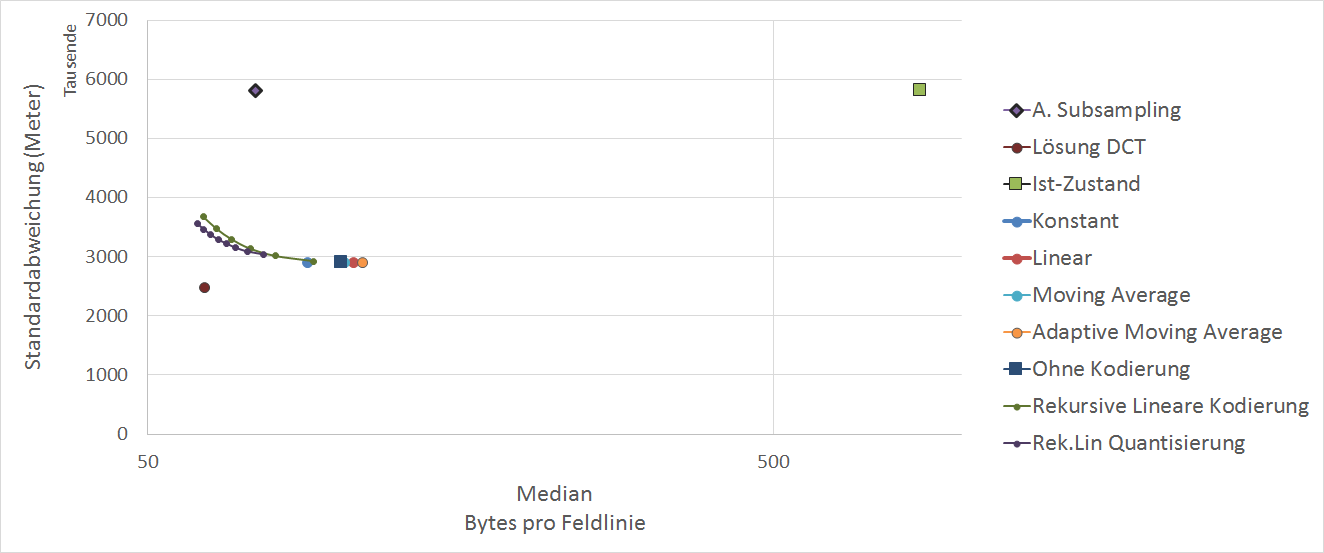
\includegraphics[width=1\textwidth,keepaspectratio]{./pictures/resultate/loesung2/variante3/resultate.png}
		\label{resultate:loesung2:adaptive:median:quant}
		\caption{Kompressionsraten der Rekursive Lineare Kodierung mit angepasster Quantisierung.}
\end{figure}
\begin{figure}[!htbp]
	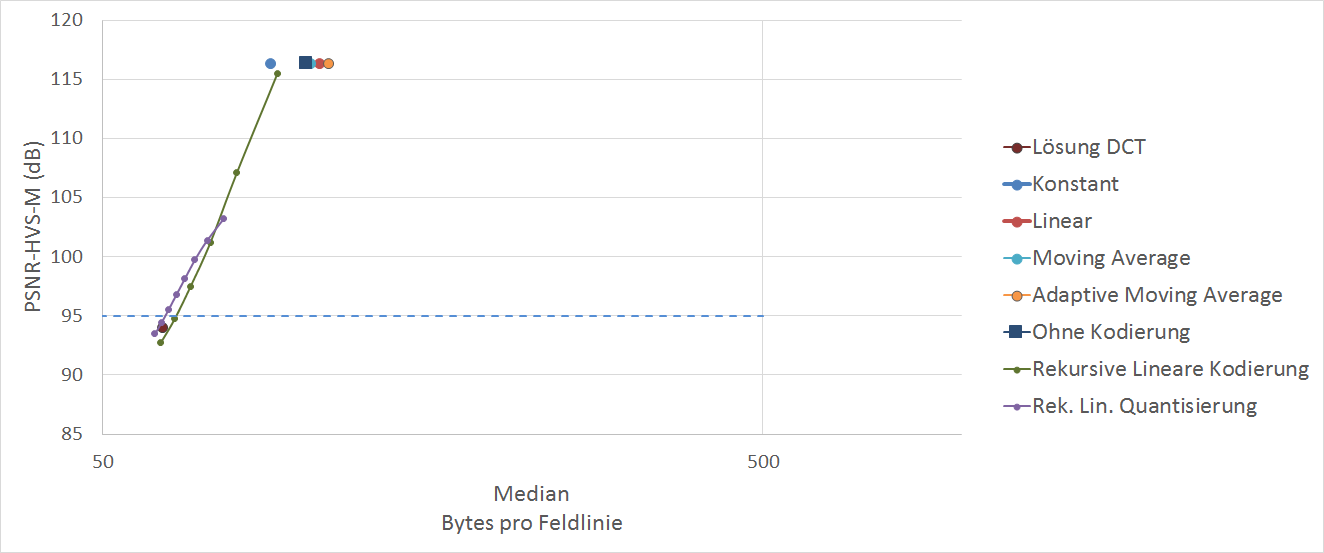
\includegraphics[width=1\textwidth,keepaspectratio]{./pictures/resultate/loesung2/variante3/resultate_psnr.png}
	\label{resultate:loesung2:adaptive:median:quant_psnr}
	\caption{Kompressionsraten der Rekursive Lineare Kodierung mit angepasster Quantisierung.}
\end{figure}
Die Angepasste Quantisierung bringt eine Verbesserung in der Standardabweichung mit sich. Die Diagramme der Abbildungen \ref{resultate:loesung2:adaptive:median:quant} und \ref{resultate:loesung2:adaptive:median:quant_psnr} visualisieren die Standardabweichung und PSNR-HVS-M zur jeweiligen Kompression. Mit der angepassten Quantisierung kann diese Variante eine ähnliche Kompression zu vergleichbaren PSNR-HVS-M erreichen, wie der DCT Lösungsansatz.Mit einer PSNR-HVS-M von $95.5$ verbraucht diese Variante $63$ Bytes pro Feldlinie, was zu einer Kompressionsrate von $13.6$ führt. Der Vorteil dieser Variante gegenüber der DCT Lösung ist, das wenige zusätzliche Bytes die Artefakten stark dämpfen können. 

Die Artefakte haben sich im Vergleich zur vorhergehenden Variante verbessert: Die Abbildung \ref{resultate:loesung2:adaptive:median_extra:artefakte}
Auch bei hohen Zoom sind die Artefakte schwer zu erkennen. Eine leichte Glättung der Feldlinien ist für die Visualisierung dennoch angebracht. Leichte Verschiebungen einzelner Punkte sind meist nicht zu erkennen. Bei hoher Dichte der Feldlinien werden die Verschiebungen sichtbar, da sie sich häufig kreuzen und eine unästhetische Visualisierung abgeben.

\begin{figure}[!htbp]
	\center
		
\includegraphics[width=0.49\textwidth,height=5cm,keepaspectratio]{./pictures/resultate/loesung2/variante3/no_artifacts.png}
	
\includegraphics[width=0.49\textwidth,height=5cm,keepaspectratio]{./pictures/resultate/loesung2/variante3/artifacts_extra.png}
	\caption{Artefakte der Rekursiven Linearen Kodierung mit angepasster Quantisierung.Links sind die originalen Feldlinien.}
	\label{resultate:loesung2:adaptive:median_extra:artefakte}
\end{figure}

Das Caching von $1000$ Simulationen und die Übertragungszeit fallen zwischen die anderen Lösungsansätzen mit $72$ Megabyte an Arbeitsspeicher beziehungsweise $58$ Sekunden Übertragungszeit. Zum Vergleich: Die DCT Lösung verbraucht unter den selben Bedingungen $70$ und das Adaptive Subsampling $85$ Megabyte an Arbeitsspeicher. Bei einer Internetverbindung von $10$ Megabit ist bei diesem Lösungsansatz mit einer Übertragungsrate von $16$ Simulationen in der Sekunde zu rechnen. Die Laufzeit der Dekompression liegt mit $30.6$ Millisekunden ebenfalls zwischen den Lösungsansätzen Adaptives Subsampling und DCT. Mit dieser Laufzeit kann ein Thread durchschnittlich $32$ Simulationen pro Sekunde dekomprimieren.

Dieser Lösungsansatz ist ein Kompromiss zwischen Kompressionsrate und Qualität. Die Daten enthalten Kompressionsartefakte. Sie sind aber schwach ausgeprägt sodass auf eine Glättung gegebenenfalls verzichtet werden kann.
